\section{波函数的统计解释}

\begin{quotation}
``不存在量子世界,只存在一个抽象的量子物理描述。''\qquad 玻尔
\end{quotation}

由de Broglie物质波假说,微观粒子的运动状态可用波函数表示,如对自由粒子,
具有确定的能量E和动量p,所以对应波函数为一个平面波:

\index{Plane wave: 平面波}

$\psi  = A\cos \left[ {k \cdot r - \omega t} \right],k = \frac{{2\pi }}{\lambda }\hat n,\omega  = 2\pi \nu $

这里$\hat n$是波动传播方向(粒子运动方向)的单位矢量。波函数一般写为复数形式:$\psi  = Ae^{i(k \cdot r - \omega t)}  = Ae^{\frac{i}{\hbar }(p \cdot r - Et)} $

\index{Wave function: 波函数}

波函数的本质:de Broglie和薛定谔认为波函数(或波包)对应的是物理实在,具有真实的物理涵义
(如把波包看作是粒子本身,或把波函数看作是原子中电荷的分布)。
玻尔等人则更倾向于把波函数看作是一种``计算方法'',看作是人们对微观粒子所具有的知识,
波函数本身不对应任何物理实在(如在经典电动力学中,\textbf{E}和\textbf{B}都对应真实的电场和磁场),无法直接测量。

\index{Wave-particle duality: 波粒二象性}

微观粒子的``波粒二象性''反映出人类认识微观规律时,宏观物理学中的概念不能完全适用,
但为了描述微观规律又不得不借用宏观物理学的语言,波、粒子、动量、能量、波长、频率,
但这些语言在微观物理学中的真实涵义已经改变,而要精确反映这些涵义的改变,
唯一的办法是使用数学语言,因为只有数学语言才是绝对精确的,
不会产生没必要的歧义
\footnote{在欧洲,很长时间以来,
拉丁语被认为是科学的语言,直到现在我们还常说法语是法律的语言。
语言是否会影响人们对客观世界的认识?不同的语言是否会导致不同的对世界的认识?
如:汉语,完全不同于西方式的语言,是``非拼音'',``单音节''的。
汉语语言的特点决定其对世界的认识是 ``诗化''的,而无法在其内部产生欧洲式的``数理''世界。
这两种对世界的认识是否是``互补''的?}。

如按照经典物理学的语言,粒子是指其具有一定的质量、电荷等属性,在空间中是集中分布的,
具有确定的位置,运动时有确定的轨道。但在微观物理学中粒子的轨道概念被彻底抛弃了,
位置也不确定了。

按经典物理学的语言,波是某种实际物理量在空间中做周期性的传播,
有干涉和衍射现象,即具有波的相干叠加性。
但在微观物理学中,物质粒子具有波动性,
并不一定要求某种实际的物理量在空间中有个分布,
但需要保留波的相干叠加性。

de Broglie和薛定谔的观点由于过分地夸大了``波''的概念,
波包的不稳定性以及我们每次观察到的都是整个电子,
而非电荷的分布。这些困难使de Broglie和薛定谔的观点没有得到大家的普遍接受。

到此为止,我们实际上仍不能回答``电子到底是粒子还是波?''
这类问题,甚至这一问题本身是否有意义都成了问题,
我们可以说电子是波、是粒子、或者什么都不是。
物理学家的任务是尽量精确地描述并预测电子的行为,
量子力学已经非常好地完成了这一任务,
至于为什么电子会这样,我们不知道。
据说当有学生问费曼``电子到底是粒子还是波?''这一问题时。
费曼的回答是``停止讨论,开始计算!''
虽然并无确切的证据说明费曼说过这样的话,但费曼确实在他的科学讲演中反复说过:
``没人理解量子力学'',``我们不打算讨论自然界为什么以她现在这种独特方式运行这类问题''
等类似观点的话\footnote{参考: 费曼《QED: 光和物质的奇异性》, pp9}。



\subsection{波函数的统计解释}

\subsubsection{波函数统计解释}

\begin{figure}[h]
\begin{center}
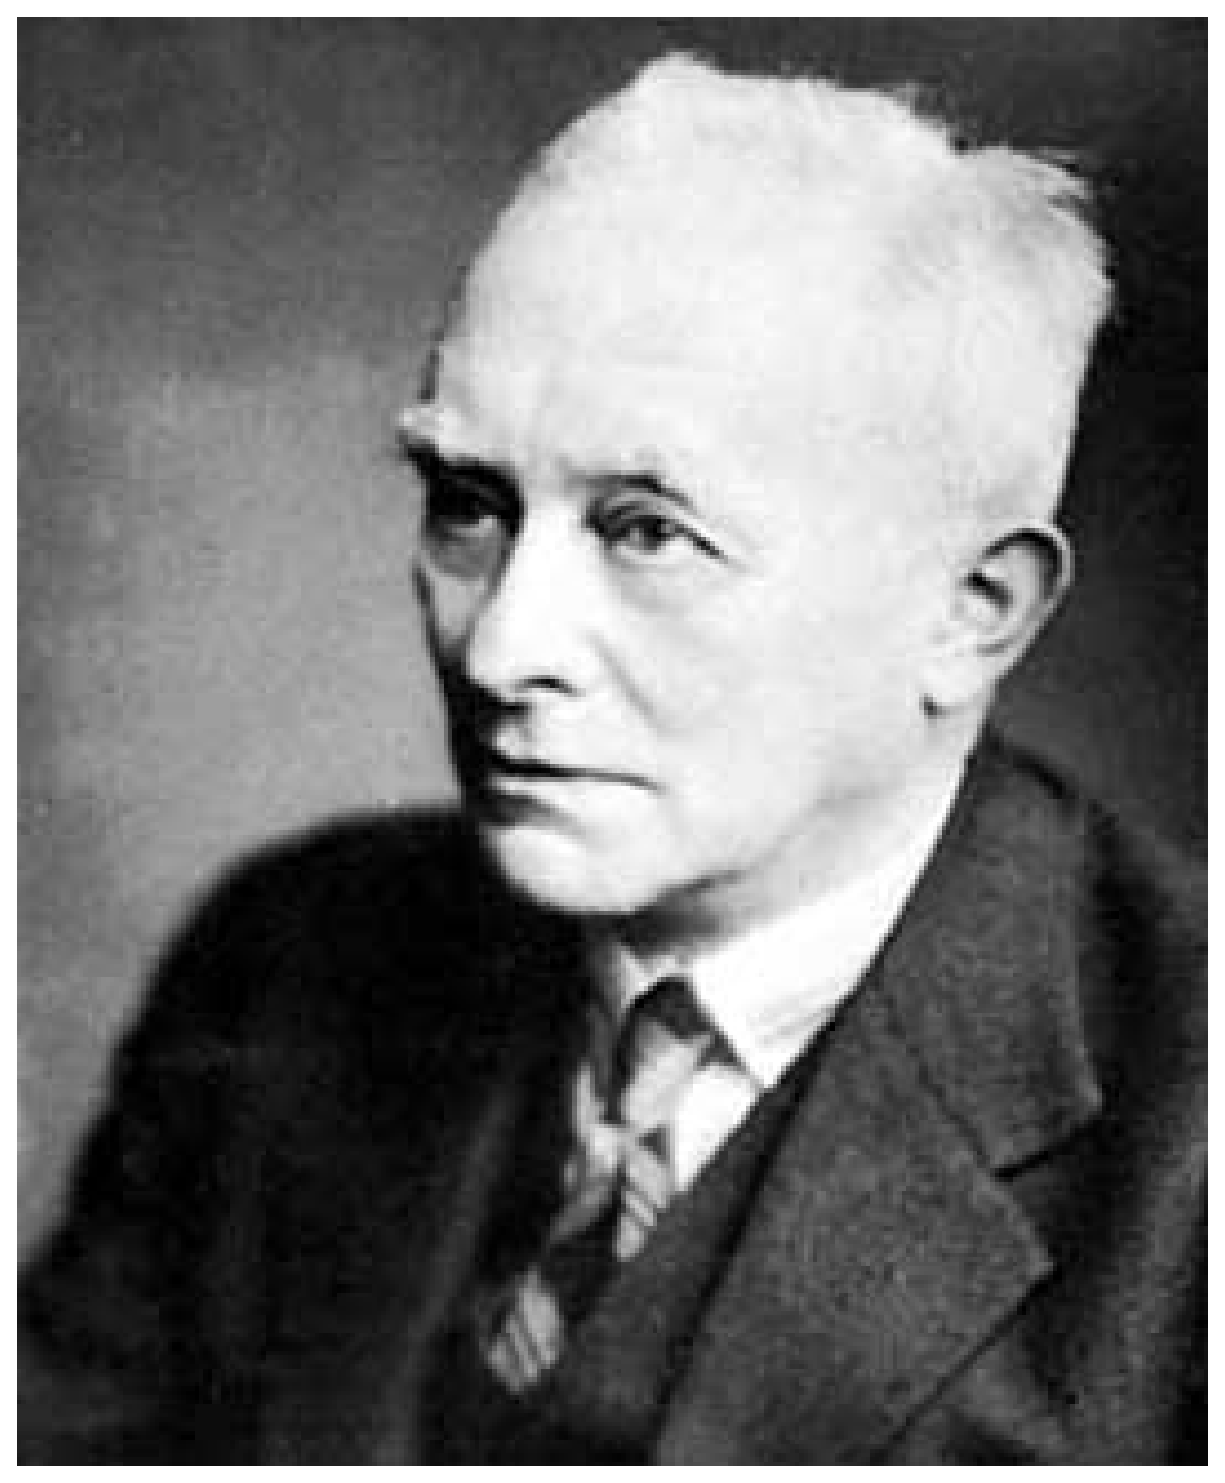
\includegraphics[clip,width=6cm]{WaveFunction/born.ps}
\caption{玻恩}
\end{center}
\end{figure}

玻恩(Max Born)提出$\left| \psi  \right|^2  = \psi \psi ^* $正比于在该点单位体积内发现粒子的几率。即:

\begin{center}
\begin{equation}\label{max born}
    w(x,y,z,t) \propto \left| {\psi (x,y,z,t)} \right|^2 d\tau
\end{equation}
\end{center}



这样物质波对应的就是几率波。

按照几率波的解释,$\psi $与$C\psi $
描述的是同样的几率分布,反映出一样多的关于微观粒子运动的信息,即描述了相同的微观粒子运动状态。

\index{Normalization: 归一化}

波函数的归一化:如微观粒子不产生,不湮没(非相对论量子力学),空间各点几率之和应为1,即:$\int_\infty  {\left| \psi  \right|^2 d\tau }  = 1$, 表示对全空间积分,满足此条件的波函数 称为归一化波函数。

\index{Square Integrable: 平方可积}

波函数的归一化条件相当于波函数的平方可积条件:$\int_\infty  {\left| \psi  \right|^2 d\tau }  = C < A$,A,C是确定正实常数。则:$\int_\infty  {\left| {\frac{\psi }{{\sqrt C }}} \right|^2 d\tau  = 1} $,即$\frac{\psi }{{\sqrt C }}$是归一化波函数,$\frac{1}{{\sqrt C }}$是归一化因子。

讨论1:相位不确定性,由于$\left| {e^{i\alpha } } \right| = 1$($\alpha$为任意实常数,相位),$e^{i\alpha } \psi $与$\psi$ 描述的是相同的微观粒子运动状态(简称为状态)。(这是因为$\psi$不对应物理实在,仅$\left| \psi  \right|^2 $对应几率波)

讨论2:一般而言,微观粒子运动状态可分为两类,束缚态(运动状态被限定在一定范围内,$E < 0$),自由态(运动状态不受限制, $E > 0$)。对束缚态,平方可积条件显然满足,但对自由态,则不成立。

\index{Bound state: 束缚态 }

\index{Free state: 自由态}

对自由粒子波函数$\psi  = Ae^{i(k \cdot r - \omega t)} $,$\left| \psi  \right|^2 $称为相对几率密度。

\textbf{例1}:箱归一化,即:我们定义波函数在边长L的立方体内是归一化的。


\index{Box normalization: 箱归一化}

\begin{center}
$\psi  = \left\{ \begin{array}{l}
 Ae^{i(k \cdot r - \omega t)} ,r \in L^3  \\
 0,r \notin L^3  \\
 \end{array} \right.$
\end{center}

对宏观材料而言,边界上的原子占材料中总原子数的比例很小,假设材料中总原子数是$N \sim  10^{24}$,那么边界上原子数$\Delta N$与总原子数的比值是:

\begin{equation}
\frac{\Delta N}{N} = 6 \frac{N^{2/3}}{N}  \sim  10^{-7} 
\end{equation}

即只有大约千万分之一,这说明边界效应很小。我们可以构造周期性边条件:

\begin{equation}
\psi (x,y,z) = \psi (x + L,y,z) = \psi (x,y + L,z) = \psi (x,y,z + L)
\end{equation}

来代替实际的边条件。上式是三维上的周期性边界条件,比较难以想象。如果是一维的话,就相当于是个首尾闭合的圆环,即我们考察的空间由$x=0$开始,到$x=L$又重新接到$x=0$上。

归一化:

\begin{equation}
\int_\infty  {\left| \psi  \right|^2 d\tau }  = \int_{V = L^3 } {A^2 d\tau }  = A^2 L^3  = 1
\end{equation}

归一化因子:

\begin{equation}
A = \frac{1}{{\sqrt V }} = \frac{1}{{\sqrt {L^3 } }}
\end{equation}

归一化波函数为:

\begin{equation}
\psi _k (r,t) = \frac{1}{{\sqrt V }}e^{i(k \cdot r - \omega t)} 
\end{equation}

周期性边界条件限制了波失$k$的取值:

\begin{equation}
k_x L = 2 n_x \pi , k_y L = 2 n_y \pi ,k_z L = 2n_z \pi 
\end{equation}

即:

\begin{equation}
k_x  = n_x \frac{{2\pi }}{L},k_y  = n_y \frac{{2\pi }}{L},k_z  = n_z \frac{{2\pi }}{L}
\end{equation}

能谱:

\begin{eqnarray*}
E &=& \hbar \omega (k) = \frac{{\hbar ^2 }}{{2m}}\left( {k_x ^2  + k_y ^2  + k_z ^2 } \right) = \frac{{p^2 }}{{2m}}  \\
{} &=& \left( {\frac{{2\pi }}{L}} \right)^2 \frac{{\hbar ^2 }}{{2m}}\left( {n_x ^2  + n_y ^2  + n_z ^2 } \right)
\end{eqnarray*}

对应自由粒子能谱。波函数可写为:

\begin{equation}
\psi _k (r,t) = \frac{1}{{\sqrt V }}\exp \left[ {i\left( {\left( {\frac{{2\pi }}{L}} \right)n \cdot r - \omega (k)t} \right)} \right] = \psi _k (r)e^{ - i\omega (k)t}
\end{equation}

这里:

\begin{equation}
\psi _k (r) = \frac{1}{{\sqrt V }}e^{ik \cdot r}  = \frac{1}{{\sqrt V }}\exp \left[ {i\left( {\frac{{2\pi }}{L}} \right)n \cdot r} \right]
\end{equation}

当$L \to \infty $时,相邻$k$值及能量值的差趋于零,看起来就是连续的了。即自由粒子对应于连续谱。


\subsubsection{正交归一}

\index{Orthonormalization: 正交归一化}

现在证明归一化波函数$\psi _k (r)$构成一个正交归一函数系,即需要证明:

\begin{equation}
\int_V {\psi _k ^* (r)\psi _{k'} (r)d^3 x}  = \left\langle {k}
 \mathrel{\left | {\vphantom {k {k'}}}
 \right. \kern-\nulldelimiterspace}
 {{k'}} \right\rangle  = \delta _{k,k'} 
\end{equation}

证明:

\begin{eqnarray*}
\left\langle {k}
 \mathrel{\left | {\vphantom {k {k'}}}
 \right. \kern-\nulldelimiterspace}
 {{k'}} \right\rangle &  = &  \frac{1}{{L^3 }}\int_{ - L/2}^{L/2} {e^{i(k'_x  - k_x )x} dx} \int_{ - L/2}^{L/2} {e^{i(k'_y  - k_y )y} dy} \int_{ - L/2}^{L/2} {e^{i(k'_z  - k_z )z} dz}  \\
{} & = & \frac{1}{{L^3 }}\int\limits_{ - L/2}^{L/2} {dxe^{i\left[ {{\textstyle{{2\pi x} \over L}}\left( {n'_x  - n_x } \right)} \right]} } \int\limits_{ - L/2}^{L/2} {dye^{i\left[ {{\textstyle{{2\pi y} \over L}}\left( {n'_y  - n_y } \right)} \right]} \int\limits_{ - L/2}^{L/2} {dze^{i\left[ {{\textstyle{{2\pi z} \over L}}\left( {n'_z  - n_z } \right)} \right]} } } \\
{} & = & \frac{1}{{L^3 }} \cdot \frac{{\sin \left( {\pi \left( {n'_x  - n_x } \right)} \right)}}{{\left( {\frac{\pi }{L}\left( {n'_x  - n_x } \right)} \right)}} \cdot \frac{{\sin \left( {\pi \left( {n'_y  - n_y } \right)} \right)}}{{\left( {\frac{\pi }{L}\left( {n'_y  - n_y } \right)} \right)}} \cdot \frac{{\sin \left( {\pi \left( {n'_z  - n_z } \right)} \right)}}{{\left( {\frac{\pi }{L}\left( {n'_z  - n_z } \right)} \right)}} \\
{} & = & \frac{{\sin \left( {\pi \left( {n'_x  - n_x } \right)} \right)}}{{\pi \left( {n'_x  - n_x } \right)}} \cdot \frac{{\sin \left( {\pi \left( {n'_y  - n_y } \right)} \right)}}{{\pi \left( {n'_y  - n_y } \right)}} \cdot \frac{{\sin \left( {\pi \left( {n'_z  - n_z } \right)} \right)}}{{\pi \left( {n'_z  - n_z } \right)}}
\end{eqnarray*}

当$n'_x  \ne n_x $时,$\sin \left[ {\left( {n'_x  - n_x } \right)\pi } \right] = 0$,当$n'_x  = n_x $时,
$\frac{{\sin \left[ {\left( {n'_x  - n_x } \right)\pi } \right]}}{{\left( {n'_x  - n_x } \right)\pi }} = 1$(通过构造$\frac{0}{0}$极限证)。

所以:

\begin{equation}
\left\langle {k}
 \mathrel{\left | {\vphantom {k {k'}}}
 \right. \kern-\nulldelimiterspace}
 {{k'}} \right\rangle  = \delta _{n_x n'_x } \delta _{n_y n'_y } \delta _{n_z n'_z }  = \delta _{kk'} 
\end{equation}

这样$\left\{ {\psi _k (r)} \right\}$就构成一个正交归一函数系。并且函数系$\left\{ {\psi _k (r)} \right\}$
是完备的,即不存在不属于$\left\{ {\psi _k (r)} \right\}$函数系,另外的某个函数$\phi (r) $与所有的$\psi _k (r)$
都正交。

$\left\{ {\psi _k (r)} \right\}$就相当于是向量空间中的一组基矢,任意波函数(相当于任意向量)可以表示为正交归一完备函数集$\left\{ {\psi
_k (r)} \right\}$ 的线性迭加:

\index{Complete orthonormal set: 正交归一完备集}

\begin{equation}
\psi  = \sum\limits_k {C_k \psi _k (r)}
\end{equation}

迭加系数$C_k$是:

\begin{equation}
C_k  = \left\langle {k}
 \mathrel{\left | {\vphantom {k \psi }}
 \right. \kern-\nulldelimiterspace}
 {\psi } \right\rangle  = \int_V {\psi _k ^* (r)\psi (r)d\tau } 
\end{equation}

\index{Hilbert Space: 希尔伯特空间}

\index{Orthonormal basis: 正交归一基}

$\psi _k (r)$也叫希尔伯特空间(Hilbert Space)中的正交归一基。希尔伯特空间是定义在复数域上的一个有限维或无限维的完备向量空间,在这个空间中定义了内积,即对线性复函数集中任一对函数$\psi (x)$和$\varphi (x)$赋予一个复数与之对应。

内积应满足以下4个条件:

\begin{enumerate}
    \item $\left\langle {\psi }
 \mathrel{\left | {\vphantom {\psi  \varphi }}
 \right. \kern-\nulldelimiterspace}
 {\varphi } \right\rangle  = \int {\psi ^* \varphi d\tau  = \left( {\int {\varphi ^* \psi d\tau } } \right)^*  = \left( {\left\langle {\varphi }
 \mathrel{\left | {\vphantom {\varphi  \psi }}
 \right. \kern-\nulldelimiterspace}
 {\psi } \right\rangle } \right)} ^* $

    \item $\left\langle {\psi }
 \mathrel{\left | {\vphantom {\psi  {\varphi _1  + \varphi _2 }}}
 \right. \kern-\nulldelimiterspace}
 {{\varphi _1  + \varphi _2 }} \right\rangle  = \left\langle {\psi }
 \mathrel{\left | {\vphantom {\psi  {\varphi _1 }}}
 \right. \kern-\nulldelimiterspace}
 {{\varphi _1 }} \right\rangle  + \left\langle {\psi }
 \mathrel{\left | {\vphantom {\psi  {\varphi _2 }}}
 \right. \kern-\nulldelimiterspace}
 {{\varphi _2 }} \right\rangle $

    \item $\left\langle {\psi }
 \mathrel{\left | {\vphantom {\psi  {C\varphi }}}
 \right. \kern-\nulldelimiterspace}
 {{C\varphi }} \right\rangle  = C\left\langle {\psi }
 \mathrel{\left | {\vphantom {\psi  \varphi }}
 \right. \kern-\nulldelimiterspace}
 {\varphi } \right\rangle $,$C$是复数;

    \item $\left\langle {\psi }
 \mathrel{\left | {\vphantom {\psi  \psi }}
 \right. \kern-\nulldelimiterspace}
 {\psi } \right\rangle  \ge 0$,仅当$\psi  = 0$时,$\left\langle {\psi }
 \mathrel{\left | {\vphantom {\psi  \psi }}
 \right. \kern-\nulldelimiterspace}
 {\psi } \right\rangle  = 0$。
   \end{enumerate}

量子力学中,微观粒子运动状态用波函数描述,
而波函数就对应希尔伯特空间\footnote{完备的内积空间就是希尔伯特空间,
关于希尔伯特空间的严格理论请阅读泛函分析方面的书籍。
如:郑维行、王声望编《实变函数与泛函分析概要》,
高等教育出版社}中的态矢量\footnote{在经典物理学中物质运动状态用位置和动量描述,而位置和动量对应于笛卡尔坐标系中的矢量。量子力学中的态矢量和经典力学中的这些矢量完全是两回事}。

由波函数归一条件:

\begin{eqnarray*}
\int_V \psi ^* \psi d\tau &=& \int_V {\left( {\sum\limits_k {C_k ^* \psi _k ^* \sum\limits_{k'} {C_{k'} \psi _{k'} } } } \right)} d\tau  \\
{} & = & \sum\limits_{k,k'} {C_k ^* C_{k'} } \int_V {\psi _k ^* \psi _{k'} d\tau } =  \sum\limits_{k,k'} {C_k ^* C_{k'} \delta _{kk'} } \\
{} & = & \sum\limits_k \left| {C_k } \right|^2  = 1
\end{eqnarray*}

$\left| {C_k } \right|^2 $就是在态矢量$\psi$中发现具有动量$p = \hbar k$粒子的几率。即:粒子动量为$\hbar k$的几率$\left| C_k \right|^2$也可由波函数求出。粒子的平均动量是:

\begin{equation}
\hbar k \left| C_k \right|^2
\end{equation}

例2:多粒子体系的波函数,$\psi (\vec r_1 ,\vec r_2 ,...,\vec r_N )$

其中:$\vec r_1 (x_1 ,y_1 ,z_1 ),\vec r_2 (x_2 ,y_2 ,z_2 ),...,\vec r_N (x_N ,y_N ,z_N )$
分别表示粒子1到粒子$N$的坐标。

归一化条件为:

\begin{equation}
\int_\infty  {\left| {\psi (\vec r_1 ,\vec r_2 ,...,\vec r_N )} \right|} ^2 d^3 \vec r_1 d^3 \vec r_2 ...d^3 \vec r_N  = 1
\end{equation}

波函数所在的希尔伯特空间和我们日常生活中的三维空间是两回事。我们后面会频繁涉及无穷多维的希尔伯特空间,但回到物理空间,我们讨论的仍然是三维空间。

\subsection{统计解释对波函数提出的要求}

\index{Wave function: 波函数}

\begin{description}
    \item[单值性:] 要求$\left| \psi  \right|$单值,但对$\psi$则不一定;
    \item[归一性:] 一个真实的波函数要求满足归一化条件,但也不排除在量子力学中可以使用一些不能归一化的理想的波函数。
如在散射理论中,常使用理想平面波函数描述入射粒子的状态,这是因为在这类问题中粒子动量基本确定,
且各处概率密度相同\footnote{参考:曾谨言《量子力学 卷I》第52页}。
    \item[对波函数奇点的要求:] 波函数的平方可积条件并不排斥在空间某些孤立奇点处$\left| {\psi (r)} \right| \to \infty $。例如,$r = r_0 $是$\psi (r)$的一个孤立奇点,$\int_{r_0  + } {\left| \psi  \right|^2 d\tau }  < M$,即波函数平方在$r_0$邻域内积分收敛。$r_0  + $表示包围$r_0$的任意小体积。


n维空间,当$dr \to 0$,$\left| \psi  \right| \to \frac{1}{{\left|
{dr} \right|^s }}$,$\left| \psi  \right|^2 (dr)^n  \to 0$,即:$n -
2s > 0$,$s < n/2$

所以对于一维,要求:$s < 1/2$;二维,$s < 1$;三维:$s < 3/2$。
即:波函数的平方可积条件限制了波函数绝对值在孤立奇点处发散的速度。

\end{description}


\subsection{测量:波函数坍缩}

我们继续对最简单的波函数:$Ae^{i\left( {kx - \omega t} \right)} $
做一些讨论,假设我们设法测量一下粒子的位置\footnote{利用超快光学测量电子运动的最新进展:
\url{http://focus.aps.org/story/v21/st7}
这里是通过制备很多相同电子波函数,
然后测量不同阶段电子的位置来获得电子运动图像的,
并非是对相同电子运动的持续测量。}。根据统计解释,
波函数绝对值平方是粒子的分布几率, 由于波函数的振幅是常数,
粒子是等几率分布的,
因此我们可能在空间中任意地方等几率地观测到粒子。那么对于一次具体的测量,
粒子将出现在何位置?我们没法预测, 只知道会在空间任何地方,
而按照经典的粒子图像,
我们总可在一定精度内测出经典粒子的位置。几率本质地出现在量子力学中,
这和经典力学决定论式的世界观有本质的区别。

暂不讨论我们是如何测量粒子位置的,
假设$t=0$时我们完成了一次成功的测量,
我们会观测到粒子在某确定位置$x=x_0$, 现在我们问:
在$t=0$之前的一瞬间粒子在什么地方?关于这个问题有两种答案\footnote{关于波函数统计解释和波函数坍缩更详尽的讨论可参考:
D. J. Griffiths, \textbf{Introduction to Quantum Mechanics},
pp2-5;}:


\textbf{答案1:} 虽然我们无法精确地知道粒子在什么地方,
但我们可推测其一定在$x_0$附近, 因为根据狭义相对论,
粒子运动速度存在一上限, 因此在测量前一瞬间,
粒子应在$x_0$附近。那么在测量前一瞬间,
波函数还是单色平面波吗?因为我们考虑的是测量前,
在此操作前波函数无任何理由发生变化,
因此应当仍然是单色平面波。但根据量子力学统计解释,
粒子应等几率地分布在整个空间,
而不是仅仅分布在$x_0$的附近。看来根据量子力学无法得到关于粒子的全部信息,
从这个角度说量子力学是不完备的。因此一定还存在某种未知因素,
决定了粒子在$x_0$附近, 因为不知道该因素到底是什么,
我们就管它叫``隐变量(Hidden variable)''。这是对量子力学的一种态度,
即认为量子力学是不完备的,
我们需要发展一种新理论取而代之。持这种观点的物理学家有爱因斯坦、玻姆等。

\textbf{答案2}:
这一派物理学家认为基于波函数和统计解释的量子力学是完备的,
我们可称之为正统派,
对创建量子力学有直接贡献的玻尔、玻恩、海森堡等都属于这一派。正统派提出``波函数坍缩(Collapse
of the wave function)''来描述量子力学的测量过程。测量前是单色平面波,
粒子等几率地处在整个空间, 一次成功的测量意味着在这一瞬间,
波函数坍缩为一位置在$x_0$附近的尖峰形函数(数学上叫$\delta$函数,
$\delta$函数仅在$x_0$取值不为$0$, 其他地方都是$0$)。根据统计解释,
粒子只能在$x_0$位置, 自然这是一次成功的测量,
因为我们得到了唯一的位置, 在$t=0$之后, 我们再做测量,
也只能获得$x_0$这一确定性的结论,
因为尖峰函数再坍缩也只能是尖峰函数。那么正统解释是否意味着与狭义相对论矛盾呢?或者说我们是否可利用波函数坍缩来构造一个可以携带信息的超过光速的信号呢?仔细的分析否定了这种设想,
但在这里我们暂不展开讨论。

\index{Collapse of the wave function: 波函数坍缩}


\begin{figure}[h]
\begin{center}
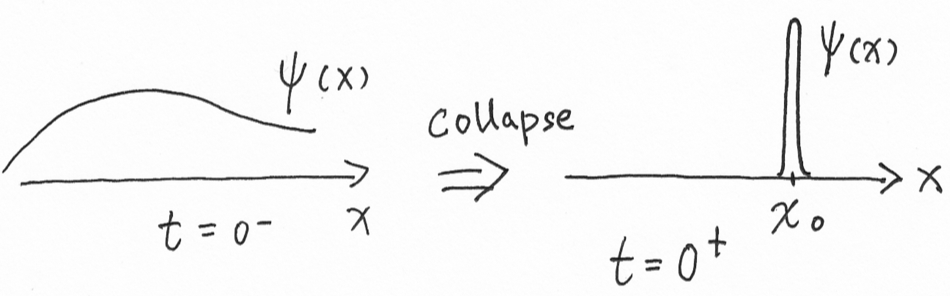
\includegraphics[clip,width=10cm]{WaveFunction/wf_collapse.png}
\caption{波函数坍缩}
\end{center}
\end{figure}

这两派意见,
到底哪一派正确呢?贝尔\footnote{关于贝尔和隐变量理论的介绍:
\url{http://gezhi.org/node/24}}后来针对隐变量理论提出了一个不等式——贝尔不等式,
如果隐变量理论成立, 不等式成立;如果正统解释成立,
则不等式可以不成立。但迄今为止的各种实验对隐变量理论都是不利的,
或者说量子力学是完备的, 波函数中包括了粒子运动的所有信息。


\subsection{波粒二象性}

\index{Wave-particle duality: 波粒二象性}

波粒二象性(Wave-particle duality)是量子力学中最核心的概念, 关于此,
最流俗的说法是: ``电子即不是粒子也不是波'',或``电子即是粒子又是波''
(这里的电子可以改为光子或其他任何东西)。``那,电子到底是什么呢?''
也许稍微改一下,就容易理解了:

\begin{itemize}
  \item 第一句改为: 电子即不是经典意义上的粒子,
  也不是经典意义上的波。
  \item 第二句改为: 电子是可以用波函数完备地描述的粒子(在量子场论中,
一般把粒子理解为场的激发)。
\end{itemize}


所谓经典意义上的粒子就是质点, 我们可用($x$, $p$)描述质点的运动,
质点满足经典力学运动规律(简单理解就是牛顿定律$F=ma$)。在经典力学意义上,
粒子的轨迹总是无限精确的, 因为原则上粒子在某一时刻,
会具有特定的位置($x$)和动量($p$)。电子当然不是经典意义上的粒子,
否则如何解释电子的双缝干涉现象。

所谓经典意义上的波动简单地理解就是机械波,
波动的能量正比于振幅的平方, 而振幅的取值是连续的,
经典的波动可以携带连续无限小的能量,
经典的波动会弥散在整个介质所在的空间。把电子看作是波动,
同样会碰到概念上的困难, 电子的稳定性会因波包的坍塌而无法解释。

所以我们说: 电子即不是经典意义上的粒子, 也不是经典意义上的波。

粒子和波动本质上是两个互相排斥的概念,
我们无法设想一个物理对象同时即是粒子又是波,
因此说电子即是粒子又是波是颇令人费解的。量子力学实际上同时打破了经典意义上的粒子和波动的图像,
它说的是: ``电子是可以用波函数完备地描述的粒子。''

理解电子到底是什么的努力将导向对波函数的讨论。因为``电子是可以用波函数完备地描述的粒子'',
在这里我们简直可以把粒子这一称谓从量子力学中去掉, 改作是
``电子可由波函数完备地描述'', 因其完备性,
我们简直可说电子就是波函数了。

根据量子力学的理论体系, 波函数是属于希尔伯特空间(Hilbert Space)
中的一个矢量, 自此我们将进入抽象的数学领域,
一方面是对波函数进行计算, 另一方面是对实验仪器进行操作,
然后我们设法把实验的结果用数学的计算进行说明。经典的粒子和波动图像完全被驱逐了,
这里倒不是说粒子和波动的图像不再被物理学家使用了,
而是说它们在新的理论体系内失去了原先的地位,
数学表达取代了日常经验中的粒子或波动的图像成为理解理论的最终落脚点。

我们会惊讶地发现, 物理学家们今天仍在使用``粒子''这一词汇,
甚至``粒子物理''作为一个重要研究领域存在着。但如前所述,
``粒子''在物理学家那里已经成为一个被抽空了意义的词汇,
我们不能对这一词汇做``理所当然、望文生义''式的理解

关于此, 费曼是这么说的\footnote{参考: 费曼《QED: 光和物质的奇异性》,
pp8-9}: ``他们(物理学家)经常以稀奇古怪的方式运用一些普通的词, 例如,
他们常常在本专业的意义上使用`功'呀、`能'呀——甚至, 你将会看到,
他们还使用`光'呀这类的词。所以当我在讲物理学上`功'的时候,
它的意思和我在街头巷尾谈论的`功劳'的`功'可不是一码事。''


\subsection{玻尔及其互补原理}

\index{Niels Bohr, 1885-1962: 玻尔}

今天如何看待玻尔在物理学史上的地位有点困难,
传统上把玻尔看作是量子力学的代言人,
玻尔和爱因斯坦对量子力学基本概念的争论曾是很轰动的事件,
被认为是科学家追求真理的象征。但玻尔不是伟大理论的创建者,
象爱因斯坦是相对论的创建者,
海森堡、薛定谔和狄拉克是量子力学的创建者,
这些基本理论的创建者当然会在物理学史上享有重要地位。今天如果我们讲授量子力学的话,
完全可以不讲玻尔模型, 直接讲授量子力学对氢原子问题的求解,
从这个角度今天以及未来的物理学家们将从课本中无时不刻地听到海森堡、薛定谔和狄拉克的名字,
但对玻尔却很少提到, 那么``玻尔到底做过什么\footnote{阅读:``The Bohr
paradox'', \url{http://physicsworld.com/cws/article/print/33963};
中译: ``玻尔之谜:如何评价玻尔的探索''
\url{http://site.douban.com/204702/widget/articles/13359152/article/26640076/}
}''这种问题就自然出现了。所以这里存在着两种逻辑,
一种是科学发现的逻辑,
另外一种是传授的逻辑。玻尔在理论传授的逻辑中是没有地位的,
但在科学发现的逻辑中则是不可缺少的一环。德布罗意(de
Broglie)正是由玻尔模型得到——``波粒二象性''(particle wave
duality)——这一建立量子力学最关键的概念。

\index{Complementarity: 互补性}

玻尔的思想有思辨色彩,
他从量子力学研究中得到``互补性(Complementarity)\footnote{玻尔自己是这么引入互补性的,
``在量子物理学中, 用不同实验装置得到的关于原子客体的资料,
却显示着一种很新颖的互补关系。事实上, 必须认识到,
这样的资料就详尽无疑地概括了关于客体的一切可设想的知识,
尽管当企图把它们结合成单独一种图景时这些资料显得是相互矛盾的。互补性这一思想绝不会限制我们以实验的形式向大自然提出问题的那些努力,
它仅仅在测量仪器和客体之间的相互作用形成现象的一个不可分割的部分时,
表征着我们通过这种询问所能接收到的答案而已。'', 摘自: 玻尔,
《尼尔斯·玻尔哲学文选》, 商务印书馆, pp233}''概念,
并努力将其推广到物理学之外的领域。但互补性仅在未建立量子力学严密体系时对理解微观物理学现象有帮助,
而一旦建立了量子力学理论体系,
互补性在其中并无任何地位。玻尔的哲学思辨某种程度上已经遮蔽了物理的思考,
比如玻尔和爱因斯坦的论战中,
爱因斯坦曾抱怨玻尔无法理解自己\footnote{参考: N. David Mermin, ``Is
the moon there when nobody looks? Reality and the quantum theory'',
\textbf{PHYSICS TODAY} / APRIL 1985 PAG. 38-47,
\url{http://www.theorie.physik.uni-konstanz.de/juan/pub/IsTheMoonThere_PhyToday38no4p38.pdf}; 部分中文翻译:
``月亮在没人看时存在吗?实在性与量子理论'',
\url{http://www.jianshu.com/p/6c304c153f6b}}。

玻尔以非凡的组织才能和迷人的感召力在他的身边汇集了当时理论物理学界最出色的年轻人,
海森堡、泡利、朗道、伽莫夫等都是玻尔的学生。玻尔的组织才能在某种程度上放大了他在物理学史上的地位,
而他与爱因斯坦的论战则起到了某种广告效应。

\subsubsection{对玻尔互补性概念的评注}

玻尔曾说: ``最终,
我们必须能将这一切解释给玛格丽特听。''玛格丽特是玻尔的妻子,
当时他正在帮助记录玻尔和其他科学家的讨论,
玛格丽特在这里代表普通人(即具有经典物理思维的人)。``互补性''可看作是玻尔努力把量子力学解释给普通人听的一种努力,
即把一套科学理论还原为``事实和逻辑''的一种努力。

一个科学理论一般包括:
公设、定义及建立在此基础上的推理论证体系。当科学理论因新的实验事实而陷入困境时,
意味着此时用于解释实验的推理论证陷入了某种逻辑上的困难。通过修正理论,
即修正概念(往往就是公设、定义)可使逻辑上的困难在新理论下不再出现。

当旧理论陷入困境, 但新理论尚未建立之时,
对困境的揭示是重要的。玻尔所强调的互补性,
其实就是对困境的明白的揭示,
是对旧理论体系下存在逻辑上困难的坦诚承认。但当新的替代性理论建立之后,
困境即告解除, 此时互补性就在新理论框架内失去了意义。

在我们的日常语言中也暗含着类似科学理论式的结构, 即也有一个包括:
公设、定义和推理体系的模糊结构, 这个结构我们不一定明确地意识到,
但当别人追问时我们就会遵循这个结构进行某种辩护。日常语言中暗含的这种结构要接受对话的考验,
它比科学理论更富有弹性, 当我们在和别人讨论问题时,
我们发现我们随时都可能在对话中修正自己的``公设、定义和推理体系'',
以应对在对话中出现的困境。但与科学理论不同的是,
在日常语言中谁也不会把这种模糊的理论体系太当真,
我们很可能在今天的对话中就对昨天刚讨论过的一个概念做完全不同的定义,
以应对今天的对话。

在相同理论框架下, 关于意义的讨论是多余的,
当(张三的)词能达(李四的)意的时候,
任何解释都是多余的。只有当不同的理论体系相遇时,
翻译和理解才显得重要。当我们把张三体系中的一段论证映射到李四体系中的一段论证时,
意义就显现了。意义是以这种相似结构,
可以用来映射的关系为基础的。有效的对话意味着存在某种翻译机制或映射机制,
使对话双方词能达意。为了达到这种词能达意的效果,
在此过程中双方有可能调整各自的理论框架(公设、定义和推理体系),
以达到可翻译, 使不理解变为可理解。

日常语言的特征是充满弹性的, 潜在地允许调整无数概念和定义,
而不致破坏日常语言本身。但科学理论则不具备这种特征,
科学理论的推理体系是刚性的, 牵一发而动全身。

比如:我们可对正义做多种定义, 甚至包括那些看上去是矛盾的定义,
而不致日常语言无法使用, 但在物理学中我们对电子的定义则要刚性得多,
是粒子、是波、还是象波一样的粒子, 这意味着整个理论结构的改变。

当我们在追求理解、追求意义的时候,
就是在从事``某种翻译的工作''。从层次的角度说, 有些是从上到下的,
有些是从下到上的, 这些都是在理解, 都是指向通达的途径和努力。
在相同理论框架内, 谈不上理解和意义, 只有推理,
自然通达。当推理陷入困境时, 我们需要追寻新的理论框架,
此时理解和意义的问题就出现了。

今天我们向普通人解释``量子力学''的困难在于,
量子力学是构建在``希尔伯特空间''基础上的,
凡是普通人需要``互补性''概念解释的地方,
量子力学都能给出一种既清晰由合乎逻辑的说法。但量子力学太抽象了,
充满了数学, 它已经不可能被翻译成日常语言了。此时,
我们再去对普通人讲量子力学的物理意义就失去了立足点。



\subsection*{阅读与思考}

\begin{itemize}
    \item 写写你对波粒二象性的认识。

参考:卢鹤绂《哥本哈根学派量子论考释》;

%德布洛意《物理学与微观物理学》,商务印书馆;

%罗森菲尔德《量子革命》,商务印书馆


\end{itemize}
